\clearpage

\begin{tcolorbox}	
\begin{tabular}{p{2.75cm} p{0.2cm} p{10.5cm}} 	
\textbf{Student Name}  &:& Tiago Esteves\\
\textbf{Starting Date} &:& October 03, 2017\\
\textbf{Goal}          &:& Implement the dimensioning of optical networks in the translucent transport mode.
\end{tabular}
\end{tcolorbox}

\section{Opaque with 1+1 Protection}
In this case study we focus on the opaque case with 1 + 1 protection. \\
The opaque transport mode performs OEO (optical-electric-optical) conversions on each intermediate node from the source to the destination node.
One advantage of this mode of transportation is that it eliminates the build up of physical deficiencies and allows for total flexibility in terms of change and cleanliness.
It can thus improve the usability of optical channels by providing grooming at each node.

\subsection{Physical Network Topology}

\subsubsection{Reference Network}
As we can see in the figure, our reference network consists of 6 nodes and 8 Bidirectional links.
The average length of the links was chosen so that the following calculations are more simplistic.

\begin{figure}[h!]
\centering
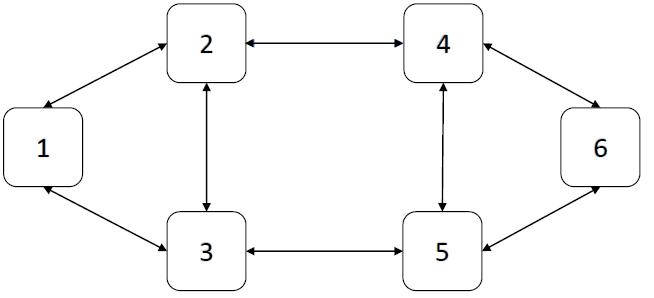
\includegraphics[width=\textwidth]{RedeTeste}
\caption{Physical Topology of the Reference Network.}
\end{figure}

\begin{table}[h!]
The following table shows the values of the variables associated with this network.\vspace{10pt}
\centering
\begin{tabular}{|| c | c | c||}
 \hline
 Constant & Description & Value \\
 \hline\hline
 N & Number of Nodes & 6 \\
 L & Number of Bidirectional Links & 8 \\
 <$\delta$> & Node out-degree & 2,667 \\
 <len> & Mean Link Length (km) & 500 \\
 <h> & Mean Number of Hops,for Working Paths & 1,533 \\
 <h'> & Mean Number of Hops,for Backup Paths & 2,467 \\
 \hline
\end{tabular}
\caption{Table of reference network values}
\label{table:1}
\end{table}

As we can see from table \ref{table:1}, to do all the calculations necessary for this project, let us know the value of the traffic used. This value is defined depending on the scenario used, as we can see:
\begin{itemize}
  \item Low Traffic: \textbf{0.5 TBits/s}
  \item High Traffic: \textbf{5 TBits/s}
\end{itemize}

\subsubsection{Realistic Network}
The real network chosen for this work is the EON (European Optical Network).
The way the nodes are arranged geographically can be seen from the following figure.

\begin{figure}[h!]
\centering
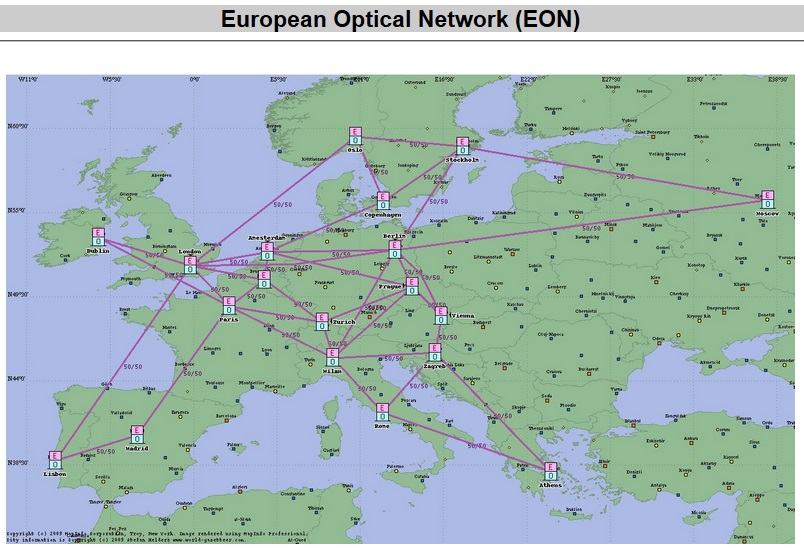
\includegraphics[width=\textwidth]{EON_Rede_Realista}
\caption{Physical Topology of the Realistic Network.}
\end{figure}

\begin{table}[h!]
The table \ref{table:2} shows the values of the variables associated with this network.\vspace{10pt}
\centering
\begin{tabular}{|| c | c | c||}
 \hline
 Constant & Description & Value \\
 \hline\hline
 N & Number of Nodes & 19 \\
 L & Number of Bidirectional Links & 37 \\
 <$\delta$> & Node out-degree & 3,89 \\
 <len> & Mean Link Length (km) & 753,76 \\
 <h> & Mean Number of Hops,for Working Paths & 2,3 \\
 <h'> & Mean Number of Hops,for Backup Paths & 3,2 \\
 \hline
\end{tabular}
\caption{Table of realistic network values}
\label{table:2}
\end{table}

Again, to make all the necessary calculations, only the value of the traffic used is missing. This value is set depending on the scenario used, as we can see:

\begin{itemize}
  \item Low Traffic: \textbf{2 TBits/s}
  \item High Traffic: \textbf{20 TBits/s}
\end{itemize}

\subsection{Dimensioning using ILP}

\subsubsection{ILP models}\label{ILP_models_OP}
The objective function of following ILP is a minimization of the sum of two variables: total number of flows crossing link (i; j) for all demand pairs (o; d) and total number of optical channels in each link (i; j).

\begin{equation}
minimize    \sum_{(i,j)} \sum_{(o,d)} f_{ij}^{od} + \sum_{(i,j)} W_{ij}
\label{ILPOpaque}
\end{equation}

$subject$ $to$
\begin{equation}
\sum_{j\textbackslash \{o\}} f_{ij}^{od} = 2  \qquad \qquad \qquad \qquad \qquad \qquad \qquad \qquad \qquad \qquad
\forall(o,d) : o < d, \forall i: i = o
\label{ILPOpaque1}
\end{equation}

\vspace{-5pt}
\begin{equation}
\sum_{j\textbackslash \{o\}} f_{ij}^{od} = \sum_{j\ \{d\}} f_{ji}^{od}   \qquad \qquad \qquad \qquad \qquad \qquad \qquad \qquad
\forall(o,d) : o < d, \forall i: i \neq o,d
\label{ILPOpaque2}
\end{equation}

\vspace{-5pt}
\begin{equation}
\sum_{j\textbackslash \{d\}} f_{ji}^{od} = 2  \qquad \qquad \qquad \qquad \qquad \qquad \qquad \qquad \qquad \qquad
\forall(o,d) : o < d, \forall i: i = d
\label{ILPOpaque3}
\end{equation}

\vspace{-5pt}
\begin{equation}
\sum_{(o,d):o<d} \left(f_{ij}^{od} + f_{ji}^{od}\right) + \sum_{c\in C} (B\left(c\right) D_{cod}\leq100 W_{ij} G_{ij} \qquad \qquad \qquad \qquad \qquad
\forall(i,j) : i < j
\label{ILPOpaque4}
\end{equation}

\vspace{-5pt}
\begin{equation}
W_{ij} \leq 80 \qquad  \qquad \qquad \qquad \qquad \qquad \qquad \qquad \qquad \qquad \qquad \qquad \qquad \forall(i,j) : i < j
\label{ILPOpaque5}
\end{equation}

\vspace{-5pt}
\begin{equation}
f_{ij}^{od} , f_{ji}^{od} \in \{0,2\}   \qquad \qquad \qquad \qquad \qquad \qquad \qquad \qquad \qquad
\forall(i,j) : i < j, \forall(o,d) : o < d
\label{ILPOpaque6}
\end{equation}

\vspace{-5pt}
\begin{equation}
W_{ij} \in \mathbb{N}  \qquad \qquad \qquad \qquad \qquad \qquad \qquad \qquad \qquad \qquad \qquad \qquad \qquad
\forall(i,j) : i < j\label{ILPOpaque7}
\end{equation}


The objective function, to be minimized, is the expression \ref{ILPOpaque}. The flow conservation constraints are \ref{ILPOpaque1}, \ref{ILPOpaque2} and \ref{ILPOpaque3}. First constraint ensures that, for all demand pairs (o,d), it routes two flows of traffic for all bidirectional links (i,j) when $j$ is not equal to the origin of the demand. Equation \ref{ILPOpaque3} is based on the same idea of \ref{ILPOpaque}, however applied in reverse direction. Assuming bidirectional traffic, so the number of flows in both directions of the link is the same \ref{ILPOpaque2}. The inequality \ref{ILPOpaque4} is considered grooming constraint, so it means the total client traffic flows can not be greater than the capacity of optical channels on all links. Another important constraint \ref{ILPOpaque5} is the capacity of the optical channels which must be less or equal to 100 Gb/s or 80 ODU0. The number of flows per demand can be zero if there are no traffic demands or two if considering working and protection traffic \ref{ILPOpaque6}. The last constraint is just needed to ensure the number optical of channels is a positive integer values greater than zero.


\subsubsection{ILP Results}

In this initial phase the results will be presented using ILP to calculate the CAPEX of the reference network.

The value of the CAPEX of the network will be calculated based on the costs of the equipment present in the figure below.
\begin{figure}[h!]
  \centering
  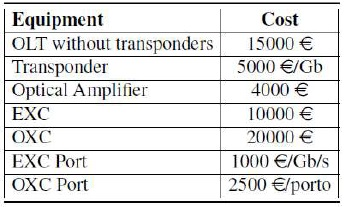
\includegraphics[scale=1]{TabValor}
  \caption{Table with costs}
  \label{TabCustOp}
\end{figure}

In addition to the equipment costs, we will also use the parameter "span", which in this case will have a value of 100.
Because this value is used to calculate the number of optical amplifiers required in the network using Equation \ref{amplifiers}.

\begin{equation}
N^R = \sum\limits_{l=1}^L\left(\left\lceil\frac{len_l}{span}\right\rceil-1\right)
\label{amplifiers}
\end{equation}

The other parameters of this equation are:
\begin{itemize}
\item{$N^R$			$\rightarrow$ Total number of regenerators/amplifiers}
\item{$len_l$		$\rightarrow$ Length of link l}
\item{$span$		$\rightarrow$ Distance between amplifiers}	
\end{itemize}	

To know the value of CAPEX it is necessary to know the value of the cost of the links and the cost of the nodes.

To calculate the cost of the nodes, the sum of the costs of the optical and electrical node is made. For this case the value of the optical cost is zero only needing to know the electric cost of the nodes that is given by equation \ref{electricalCostOpaque}.

\begin{equation}
C_{exc} = \left(\gamma_{e0}\times N\right) + \gamma_{e1} \times \left(T_1 + \left(2 \times w^0 \times \tau \right)\right)
\label{electricalCostOpaque}
\end{equation}

\begin{itemize}
\item{$C_{exc}$		$\rightarrow$	Electrical Ports Cost}
\item{$\gamma_{e0}$	$\rightarrow$	EXC cost in Euros}
\item{$N$			$\rightarrow$	Number of Nodes}
\item{$\gamma_{e1}$	$\rightarrow$	EXC port cost in Euros}
\item{$T_1$         $\rightarrow$   Total Unidirectional Traffic}
\item{$w^0$			$\rightarrow$	Total number of optical channels}
\item{$\tau$		$\rightarrow$	Traffic per port}
\end{itemize}

To calculate the cost of the Links we will use the equation \ref{linkCosts}.

\begin{equation}
C_L = \left(\gamma_0^{OLT} \times L\right) + \left(\gamma_1^{OLT} \times \tau \times W\right) + \left(N^R \times c^R\right)
\label{linkCosts}
\end{equation}	
	
\begin{itemize}
\item{$C_L$				$\rightarrow$	Links Cost}
\item{$\gamma_0^{OLT}$	$\rightarrow$	OLT cost in Euros}
\item{$L$				$\rightarrow$	Number of unidirectional Links}
\item{$\gamma_1^{OLT}$	$\rightarrow$	Transponder cost in Euros}
\item{$W$             $\rightarrow$	Total number of optical channels}
\item{$N^R$				$\rightarrow$	Total number of optical amplifiers}
\item{$c^R$				$\rightarrow$	Optical amplifiers cost in Euros}
\end{itemize}

To perform the calculations using the implementation of the models described in section \ref{ILP_models_OP} it is necessary to use a mathematical software tool. For this we will use MATLAB which is ideal for dealing with linear programming problems and can call the LPsolve through an external interface.

\pagebreak
Using the values calculated through MatLab as well as the values indicated in table \ref{table:1} or table \ref{table:2} (depending on the scenario used) and figure \ref{TabCustOp} we can finally calculate the CAPEX value using equations \ref{electricalCostOpaque} and \ref{linkCosts} for the various situations mentioned.\\

\textbf{Low Traffic scenario:}\\

$C_L$ = \textbf{24 336 000\euro}

$C_N$ = $C_{exc}$ = \textbf{5 860 000\euro}

$CAPEX$ = 24 336 000 + 5 860 000 = \textbf{30 196 000\euro}\\

\textbf{High Traffic scenario:}\\

$C_L$ = \textbf{191 336 000\euro}

$C_N$ = $C_{exc}$ = \textbf{48 260 000 \euro}

$CAPEX$ = 191 336 000 + 48 260 000 = \textbf{239 596 000 \euro}\\

\subsection{Dimensioning using Heuristics}

\subsubsection{Heuristics Models}

\subsubsection{Heuristics Results}

\subsection{Analysis and comparison of results}
